\scanpage{58}
% archive sheet number: 57

% L1–8, example 4
\uline{Exemple 4} \unsure{Donnons|Donnant} un contre-exemple à la question du début. $Y$ est formé de deux courbes irréductibles \inserted{$Y_1,Y_2$} se coupant en 2 pts $a,b$, dans $X$ irréductible. $F$ est le faisceau des applications de $X$ dans $\mathbb{Q}$. \deleted{On a} \unsure{Cons.|On a} la suite exacte

% L4–8, upper left
\figure{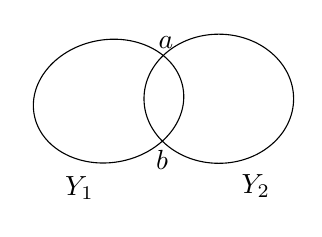
\begin{tikzpicture}[x=1cm,y=1cm]\draw[rotate=10] (0,0) ellipse (.96 and .78);\draw (1.40,.03) ellipse (.95 and .82);\node[above] at (.73,.54) {$a$};\node[below] at (.68,-.50) {$b$};\node[below] at (-.37,-.83) {$Y_1$};\node[below] at (1.87,-.81) {$Y_2$};\end{tikzpicture}}

% L9, cohomology sequence
\[
H^0(Y_1,F_1)\times H^0(Y_2,F_{Y_2})\longrightarrow
\underset{\substack{\deleted{\unsure{H}}\ \shortparallel\\F_a\times F_b}}{H^0(Y_{12},\deleted{\unsure{F_{Y_{12}}}} F_{12})}
\mathbin{\unsure{-|\to}}H^1(Y,F_Y)\longrightarrow0
\]

% L10–15, explanation
[$F_i=F_{Y_i},\ \unsure{F_{12}|H_{12}}=F_{Y_{12}}$] donc la question est de représenter un élément de $H^0(Y_{12},F_{12})=F_a\times F_b$ comme \uline{différence} $f_1-f_2$, où $f_i\in H^0(Y_i,F_i)$. \unsure{Je prend|On prend} l'élmt $(0,1)\in F_a\times F_b$, je dis qu'il ne se représente pas comme diff.

% L16–22, proof and overwritten line
En effet, si on avait une solution $f_1,f_2$, on aurait un voisinage $U$ \inserted{($U'$)} de $a$ \inserted{($b$)}, et \deleted{\unsure{$\varphi,\varphi'$}} tel \deleted{\unsure{que,} \unsure{$\varphi$}} $\unsure{\varphi|\phi}_1,\varphi_2\in\Gamma(U,F)$ \deleted{\unsure{\,$\varphi,\varphi'\in\Gamma(U,F)$}} [$\varphi'_1,\varphi'_2\in\Gamma(U,F)$] \deleted{\unsure{$\varphi',\varphi'\in\Gamma$}} tels que pour tt $x\in Y_i\cap U$, on ait $f_{ix}=\varphi_{ix}$ ($x\in Y_i\cap U'$ on ait $f_{ix}=\varphi'_{ix}$). De plus, prenant $U$ ($U'$) assez petits, on devra avoir \deleted{\unsure{$f$}} $\varphi_2\unsure{-|=}\varphi_1=0$ [resp. $\varphi'_2-\varphi'_1=1$] ;

% L22–26, heavily crossed lower continuation
\deleted{alors, prenant \unsure{de un} alors un fermé de $X$ ne contenant pas \unsure{qui} tt pt de $x\in Y_1\cap U\cap U'$ \unsure{assez} au \unsure{autre} $a$ ni $b$ [réunion d'un voisinage de $Y_1$ et d'un voisinage de $Y_2$] on devra avoir} On aura alors $\varphi_{1x}=\varphi'_{\unsure{1|2}x}$ \deleted{$(=f_{1x})$, \unsure{et voir}} pour $x\in$
